%% fig_charactergrid.tex   (generated by make_core.py; do not edit by hand)
%% The K-grading of H^{2n} at n = 3: the summand at (r,s) with its true dimension, and the three cells that matter.
\documentclass[tikz,border=8pt]{standalone}
\usepackage{amsmath,amssymb}
\usetikzlibrary{arrows.meta,calc}
%% palette.tex -- shared colour definitions for the figures
\definecolor{PInk}{RGB}{26,32,44}
\definecolor{PBlue}{RGB}{37,82,139}
\definecolor{PTeal}{RGB}{23,127,125}
\definecolor{POchre}{RGB}{193,138,44}
\definecolor{PClay}{RGB}{178,74,58}
\definecolor{PSlate}{RGB}{108,122,137}
\definecolor{PViolet}{RGB}{110,86,150}
\definecolor{WBlue}{RGB}{223,234,246}
\definecolor{WTeal}{RGB}{220,238,236}
\definecolor{WOchre}{RGB}{250,240,218}
\definecolor{WClay}{RGB}{247,229,224}
\definecolor{WSlate}{RGB}{238,241,244}
\definecolor{PMag}{RGB}{158,58,110}
\definecolor{PGrass}{RGB}{62,124,66}
\definecolor{PAmber}{RGB}{214,112,38}
\definecolor{PIndigo}{RGB}{58,64,140}
\definecolor{PRule}{RGB}{176,186,197}

%% shared macros so the standalone figures match the paper
\providecommand{\QQ}{\mathbb{Q}}
\providecommand{\ZZ}{\mathbb{Z}}
\providecommand{\RR}{\mathbb{R}}
\providecommand{\CC}{\mathbb{C}}
\providecommand{\PP}{\mathbb{P}}
\providecommand{\Kx}{K^{\times}}
\providecommand{\HW}{W}
\providecommand{\Nm}{\mathrm{N}}
\providecommand{\Hdg}{\mathrm{Hdg}}
\providecommand{\NS}{\mathrm{NS}}
\providecommand{\cA}{\mathcal{A}}
\providecommand{\cD}{\mathcal{D}}
\providecommand{\cF}{\mathcal{F}}
\providecommand{\cP}{\mathcal{P}}
\providecommand{\cO}{\mathcal{O}}
\providecommand{\cQ}{\mathcal{Q}}
\providecommand{\bbar}[1]{\overline{#1}}
\providecommand{\ch}{\operatorname{ch}}
\providecommand{\End}{\mathrm{End}}

\begin{document}
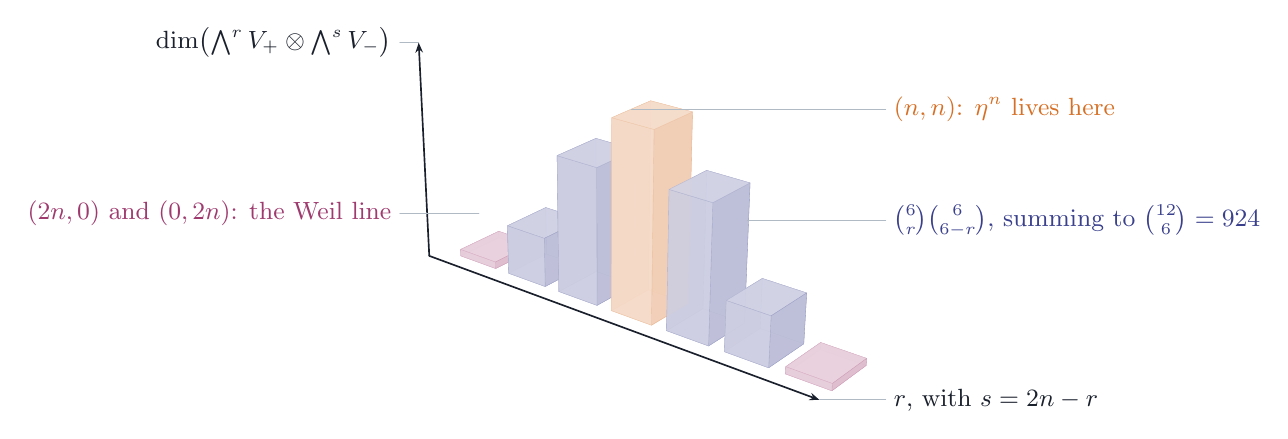
\begin{tikzpicture}[x=1cm,y=1cm,line join=round,line cap=round,
  font=\small,text=PInk]
  \path[draw=PMag!41!white,line width=0.12pt,fill opacity=0.90,fill=PMag!25!white] (-1.3490,0.0615) -- (-0.9102,-0.0913) -- (-0.9119,-0.0102) -- (-1.3514,0.1417) -- cycle;
  \path[draw=PMag!50!white,line width=0.12pt,fill opacity=0.90,fill=PMag!34!white] (-1.8334,-0.1711) -- (-1.3490,0.0615) -- (-1.3514,0.1417) -- (-1.8367,-0.0894) -- cycle;
  \path[draw=PMag!39!white,line width=0.12pt,fill opacity=0.90,fill=PMag!23!white] (-1.8334,-0.1711) -- (-1.3917,-0.3317) -- (-0.9102,-0.0913) -- (-1.3490,0.0615) -- cycle;
  \path[draw=PMag!39!white,line width=0.12pt,fill opacity=0.90,fill=PMag!23!white] (-1.8367,-0.0894) -- (-1.3943,-0.2489) -- (-0.9119,-0.0102) -- (-1.3514,0.1417) -- cycle;
  \path[draw=PMag!50!white,line width=0.12pt,fill opacity=0.90,fill=PMag!34!white] (-1.3917,-0.3317) -- (-0.9102,-0.0913) -- (-0.9119,-0.0102) -- (-1.3943,-0.2489) -- cycle;
  \path[draw=PMag!41!white,line width=0.12pt,fill opacity=0.90,fill=PMag!25!white] (-1.8334,-0.1711) -- (-1.3917,-0.3317) -- (-1.3943,-0.2489) -- (-1.8367,-0.0894) -- cycle;
  \path[draw=PIndigo!41!white,line width=0.12pt,fill opacity=0.90,fill=PIndigo!25!white] (-0.7450,-0.1489) -- (-0.2863,-0.3088) -- (-0.2901,0.2908) -- (-0.7548,0.4428) -- cycle;
  \path[draw=PIndigo!50!white,line width=0.12pt,fill opacity=0.90,fill=PIndigo!34!white] (-1.2252,-0.3922) -- (-0.7450,-0.1489) -- (-0.7548,0.4428) -- (-1.2418,0.2114) -- cycle;
  \path[draw=PIndigo!39!white,line width=0.12pt,fill opacity=0.90,fill=PIndigo!23!white] (-1.2252,-0.3922) -- (-0.7629,-0.5603) -- (-0.2863,-0.3088) -- (-0.7450,-0.1489) -- cycle;
  \draw[PInk,line width=0.6pt,-{Stealth[length=3.6pt]}] (-2.2347,-0.1708) -- (-2.3691,2.5376);
  \path[draw=PIndigo!39!white,line width=0.12pt,fill opacity=0.90,fill=PIndigo!23!white] (-1.2418,0.2114) -- (-0.7734,0.0514) -- (-0.2901,0.2908) -- (-0.7548,0.4428) -- cycle;
  \path[draw=PIndigo!50!white,line width=0.12pt,fill opacity=0.90,fill=PIndigo!34!white] (-0.7629,-0.5603) -- (-0.2863,-0.3088) -- (-0.2901,0.2908) -- (-0.7734,0.0514) -- cycle;
  \path[draw=PIndigo!41!white,line width=0.12pt,fill opacity=0.90,fill=PIndigo!25!white] (-1.2252,-0.3922) -- (-0.7629,-0.5603) -- (-0.7734,0.0514) -- (-1.2418,0.2114) -- cycle;
  \path[draw=PIndigo!39!white,line width=0.12pt,fill opacity=0.90,fill=PIndigo!23!white] (-0.5886,-0.6237) -- (-0.1041,-0.7998) -- (0.3667,-0.5363) -- (-0.1134,-0.3690) -- cycle;
  \path[draw=PIndigo!41!white,line width=0.12pt,fill opacity=0.90,fill=PIndigo!25!white] (-0.1134,-0.3690) -- (0.3667,-0.5363) -- (0.3808,1.1773) -- (-0.1177,1.3212) -- cycle;
  \path[draw=PIndigo!50!white,line width=0.12pt,fill opacity=0.90,fill=PIndigo!34!white] (-0.5886,-0.6237) -- (-0.1134,-0.3690) -- (-0.1177,1.3212) -- (-0.6114,1.1021) -- cycle;
  \path[draw=PAmber!39!white,line width=0.12pt,fill opacity=0.90,fill=PAmber!23!white] (0.0786,-0.8663) -- (0.5868,-1.0511) -- (1.0507,-0.7747) -- (0.5477,-0.5994) -- cycle;
  \path[draw=PIndigo!50!white,line width=0.12pt,fill opacity=0.90,fill=PIndigo!34!white] (-0.1041,-0.7998) -- (0.3667,-0.5363) -- (0.3808,1.1773) -- (-0.1083,0.9503) -- cycle;
  \path[draw=PIndigo!41!white,line width=0.12pt,fill opacity=0.90,fill=PIndigo!25!white] (-0.5886,-0.6237) -- (-0.1041,-0.7998) -- (-0.1083,0.9503) -- (-0.6114,1.1021) -- cycle;
  \path[draw=PAmber!41!white,line width=0.12pt,fill opacity=0.90,fill=PAmber!25!white] (0.5477,-0.5994) -- (1.0507,-0.7747) -- (1.1083,1.6577) -- (0.5772,1.7986) -- cycle;
  \path[draw=PIndigo!39!white,line width=0.12pt,fill opacity=0.90,fill=PIndigo!23!white] (-0.6114,1.1021) -- (-0.1083,0.9503) -- (0.3808,1.1773) -- (-0.1177,1.3212) -- cycle;
  \path[draw=PAmber!50!white,line width=0.12pt,fill opacity=0.90,fill=PAmber!34!white] (0.0786,-0.8663) -- (0.5477,-0.5994) -- (0.5772,1.7986) -- (0.0830,1.5840) -- cycle;
  \draw[PInk,line width=0.6pt,-{Stealth[length=3.6pt]}] (-2.2347,-0.1708) -- (2.7212,-2.0005);
  \path[draw=PIndigo!39!white,line width=0.12pt,fill opacity=0.90,fill=PIndigo!23!white] (0.7787,-1.1208) -- (1.3124,-1.3149) -- (1.7681,-1.0247) -- (1.2405,-0.8409) -- cycle;
  \path[draw=PIndigo!41!white,line width=0.12pt,fill opacity=0.90,fill=PIndigo!25!white] (1.2405,-0.8409) -- (1.7681,-1.0247) -- (1.8394,0.7561) -- (1.2896,0.9149) -- cycle;
  \path[draw=PIndigo!50!white,line width=0.12pt,fill opacity=0.90,fill=PIndigo!34!white] (0.7787,-1.1208) -- (1.2405,-0.8409) -- (1.2896,0.9149) -- (0.8104,0.6731) -- cycle;
  \path[draw=PAmber!50!white,line width=0.12pt,fill opacity=0.90,fill=PAmber!34!white] (0.5868,-1.0511) -- (1.0507,-0.7747) -- (1.1083,1.6577) -- (0.6199,1.4350) -- cycle;
  \path[draw=PAmber!41!white,line width=0.12pt,fill opacity=0.90,fill=PAmber!25!white] (0.0786,-0.8663) -- (0.5868,-1.0511) -- (0.6199,1.4350) -- (0.0830,1.5840) -- cycle;
  \path[draw=PIndigo!41!white,line width=0.12pt,fill opacity=0.90,fill=PIndigo!25!white] (1.9673,-1.0942) -- (2.5214,-1.2873) -- (2.5585,-0.6413) -- (1.9957,-0.4572) -- cycle;
  \path[draw=PIndigo!50!white,line width=0.12pt,fill opacity=0.90,fill=PIndigo!34!white] (1.5140,-1.3882) -- (1.9673,-1.0942) -- (1.9957,-0.4572) -- (1.5365,-0.7376) -- cycle;
  \path[draw=PIndigo!39!white,line width=0.12pt,fill opacity=0.90,fill=PIndigo!23!white] (1.5140,-1.3882) -- (2.0753,-1.5923) -- (2.5214,-1.2873) -- (1.9673,-1.0942) -- cycle;
  \path[draw=PIndigo!50!white,line width=0.12pt,fill opacity=0.90,fill=PIndigo!34!white] (1.3124,-1.3149) -- (1.7681,-1.0247) -- (1.8394,0.7561) -- (1.3668,0.5051) -- cycle;
  \path[draw=PAmber!39!white,line width=0.12pt,fill opacity=0.90,fill=PAmber!23!white] (0.0830,1.5840) -- (0.6199,1.4350) -- (1.1083,1.6577) -- (0.5772,1.7986) -- cycle;
  \path[draw=PIndigo!41!white,line width=0.12pt,fill opacity=0.90,fill=PIndigo!25!white] (0.7787,-1.1208) -- (1.3124,-1.3149) -- (1.3668,0.5051) -- (0.8104,0.6731) -- cycle;
  \path[draw=PMag!41!white,line width=0.12pt,fill opacity=0.90,fill=PMag!25!white] (2.7307,-1.3602) -- (3.3132,-1.5632) -- (3.3201,-1.4726) -- (2.7362,-1.2709) -- cycle;
  \path[draw=PIndigo!39!white,line width=0.12pt,fill opacity=0.90,fill=PIndigo!23!white] (1.5365,-0.7376) -- (2.1067,-0.9324) -- (2.5585,-0.6413) -- (1.9957,-0.4572) -- cycle;
  \path[draw=PIndigo!39!white,line width=0.12pt,fill opacity=0.90,fill=PIndigo!23!white] (0.8104,0.6731) -- (1.3668,0.5051) -- (1.8394,0.7561) -- (1.2896,0.9149) -- cycle;
  \path[draw=PIndigo!50!white,line width=0.12pt,fill opacity=0.90,fill=PIndigo!34!white] (2.0753,-1.5923) -- (2.5214,-1.2873) -- (2.5585,-0.6413) -- (2.1067,-0.9324) -- cycle;
  \path[draw=PMag!50!white,line width=0.12pt,fill opacity=0.90,fill=PMag!34!white] (2.2874,-1.6695) -- (2.7307,-1.3602) -- (2.7362,-1.2709) -- (2.2922,-1.5782) -- cycle;
  \path[draw=PIndigo!41!white,line width=0.12pt,fill opacity=0.90,fill=PIndigo!25!white] (1.5140,-1.3882) -- (2.0753,-1.5923) -- (2.1067,-0.9324) -- (1.5365,-0.7376) -- cycle;
  \path[draw=PMag!39!white,line width=0.12pt,fill opacity=0.90,fill=PMag!23!white] (2.2874,-1.6695) -- (2.8784,-1.8843) -- (3.3132,-1.5632) -- (2.7307,-1.3602) -- cycle;
  \path[draw=PMag!39!white,line width=0.12pt,fill opacity=0.90,fill=PMag!23!white] (2.2922,-1.5782) -- (2.8846,-1.7918) -- (3.3201,-1.4726) -- (2.7362,-1.2709) -- cycle;
  \path[draw=PMag!50!white,line width=0.12pt,fill opacity=0.90,fill=PMag!34!white] (2.8784,-1.8843) -- (3.3132,-1.5632) -- (3.3201,-1.4726) -- (2.8846,-1.7918) -- cycle;
  \path[draw=PMag!41!white,line width=0.12pt,fill opacity=0.90,fill=PMag!25!white] (2.2874,-1.6695) -- (2.8784,-1.8843) -- (2.8846,-1.7918) -- (2.2922,-1.5782) -- cycle;
  \draw[PRule,line width=0.35pt] (-2.6091,2.5376) -- (-2.3691,2.5376);
  \node[anchor=east,inner sep=0pt] at (-2.7091,2.5376) {$\dim\bigl(\bigwedge^{r}V_{+}\otimes\bigwedge^{s}V_{-}\bigr)$};
  \draw[PRule,line width=0.35pt] (-2.6091,0.3723) -- (-1.6032,0.3723);
  \node[text=PMag,anchor=east,inner sep=0pt] at (-2.7091,0.3723) {$(2n,0)$ and $(0,2n)$: the Weil line};
  \draw[PRule,line width=0.35pt] (3.5601,1.6928) -- (0.3335,1.6928);
  \node[text=PAmber,anchor=west,inner sep=0pt] at (3.6601,1.6928) {$(n,n)$: $\eta^{n}$ lives here};
  \draw[PRule,line width=0.35pt] (3.5601,0.2731) -- (1.8038,0.2731);
  \node[text=PIndigo,anchor=west,inner sep=0pt] at (3.6601,0.2731) {$\binom{6}{r}\binom{6}{6-r}$, summing to $\binom{12}{6}=924$};
  \draw[PRule,line width=0.35pt] (3.5601,-2.0005) -- (2.7212,-2.0005);
  \node[anchor=west,inner sep=0pt] at (3.6601,-2.0005) {$r$, with $s=2n-r$};
\end{tikzpicture}
\end{document}
